\chapter{Model Inference and Revision}
When modeling a real system, it is usually demanded to assess the correctness of a Boolean network with the concrete system by checking if the observed configurations are indeed reachable in the Boolean network.
Whenever it is not the case, it typically means that the designed Boolean functions do not model the given system correctly, and thus should be revised before further model analysis.

\section{Model Inference via Statistics}

\subsection{P-value and Partial Correlation}
A drawback of previous approaches is that it needs hypotheses (possible regulations). In case of networks of big scale, it is not possible to calculate hypotheses by hand nor traverse all the possible addable actions, as stated formerly, verification of  $\mathcal{O}(3^{|Global States|})$ states is a huge task (for any component, each of other components has 3 possibilities, promotion, inhibition and no regulation).\par
To deal with the great complexity of verification of states, prior knowledge is needed. It reduces the amount of states to be verified.  statistical approaches come into sight,
Also, original time series data are discretized before being used in the last section, 
Also, the data used in last section are not ``original'' as they are discretized. Considering the complexity of verification of hypotheses and making full use of these data, statistical approaches are considered in generation of possible regulations before discretization.\par

\begin{figure}[ht]
\centering
\begin{tikzpicture}[node distance = 1.5cm, auto]
    % Place nodes
    \node [block] (originalData) {original data};
    \node [block, right = of originalData] (dataDiscretization) {data discretization};
     \node [block, right = of dataDiscretization] (varReconstruction) {variable reconstruction};
    \node [block, below = of originalData] (ranking) {ranking};
    \node [block, right = of ranking] (changeRate) {change rate};
    \node [block, below = of ranking] (dataReg) {data regrouping \& Spearman coefficient};
     \node [block, right = of dataReg] (partialCoeff) {partial coefficient};
     \node [block, right = of partialCoeff] (regulations) {regulations $x\xrightarrow{+/-}y$};
     \node [block, below = of varReconstruction] (actions) {actions \ac{x_i}{y_j}{y_k}};
     \coordinate [left = of ranking,node distance=0.5cm](abstract);
    % Draw edges
    \path [line] (originalData) -- (dataDiscretization);
    \path [line] (originalData) -- (ranking);
    \path [line] (originalData) -- (changeRate);
    \path [line] (changeRate) -- (ranking);
    \path [line,dashed] (dataDiscretization) -- (varReconstruction);
    \path [line] (varReconstruction) -- (ranking);
    \path [line] (ranking) -- (dataReg);
    \path [line] (dataReg) -- (partialCoeff);
    \path [line] (partialCoeff) -- (regulations);
    \path [line,dashed] (regulations) -- (actions);
    \path [line,dashed] (originalData) -|  (abstract)node[rotate=90,below=2pt]{Pearson Coefficient} |-(dataReg);
\end{tikzpicture}
\caption{Workflow of the whole procedure of hypotheses generation (dashed arrows stand for optional processes)}\label{plan}
\end{figure}
Figure \ref{plan} shows the procedure of regulation generation: before discretizing original data, Pearson or Spearman correlation coefficient \cite{samaga2009logic,hauke2011comparison} are calculated for identifying the relevance between original data and change rates of components (in linear or monotonic way respectively). If cooperation between components exists, former coefficients need replacing by partial ones \cite{de2004discovery} for more precise result. High resulting coefficients (an arbitrary threshold of relevance can be set, e.g.  0.8) suggest the add of regulations.\par
Furthermore, to complete BRN in form of Process Hitting, more accurate regulations are inferred through variable reconstruction, which splits a variable into several new variable according to its qualitative levels, e.g. component $a$ has two levels $a_0$ $a_1$, then correlation coefficients as well as partial coefficients are calculated in the domain of $a_0$ and of $a_1$ separately. As a result, the relevance between $a_0$ and other components and that of $a_1$ are calculated, with which possible addable actions of Process Hitting are deduced.\par
As all the subroutines depicted in Figure \ref{plan} are implemented, starting from original data, regulations in form of Thomas' model or Process Hitting are resulted step by step. In the next, the data treatments Figure \ref{plan} will be introduced with examples.

%\subsection{Partial Correlation Coefficients}
\subsection{Data Regrouping}
To gain an understanding of correlations between observation data and change rate, certain observed data of one component are replaced by corresponding change rate. By calculating the correlation coefficients of such matrix, regulation on this component is characterized.\par
Example:\par
$$\kbordermatrix{\mbox{}&t_0&t_1&t_2&t_3\\
a&a_{t_0}&a_{t_1}&a_{t_2}&a_{t_3}\\
b&b_{t_0}&b_{t_1}&b_{t_2}&b_{t_3}\\
c&c_{t_0}&c_{t_1}&c_{t_2}&c_{t_3}\\
d&d_{t_0}&d_{t_1}&d_{t_2}&d_{t_3}
}
\to\kbordermatrix{\mbox{}&t_0&t_1&t_2\\
a'&a'_{t_0}&a'_{t_1}&a'_{t_2}\\
b&b_{t_0}&b_{t_1}&b_{t_2}\\
c&c_{t_0}&c_{t_1}&c_{t_2}\\
d&d_{t_0}&d_{t_1}&d_{t_2}
}$$

With delay = 1 time unit, $a'$ is the change rate of $a$, calculated via 
$$a'=\dfrac{\mathrm{d}a(t)}{\mathrm{d}t}=\dfrac{a(t+1)-a(t)}{(t+1)-t}=a(t+1)-a(t)$$ In this way, regulations of $b,c,d$ on $a$ are then evaluated by aforementioned coefficients. Also matrices representing different delays can be formed likewise.
\subsection{Inference of Different Delay using Variable Reconstruction}
By applying aforementioned approaches, regulations in the form of $a\xrightarrow{+/-}b$ are deduced, but the result is not in the precise form of Process Hitting. To obtain a result in such form, variable reconstruction is compulsory. \par
\begin{figure}[!ht]
\centering
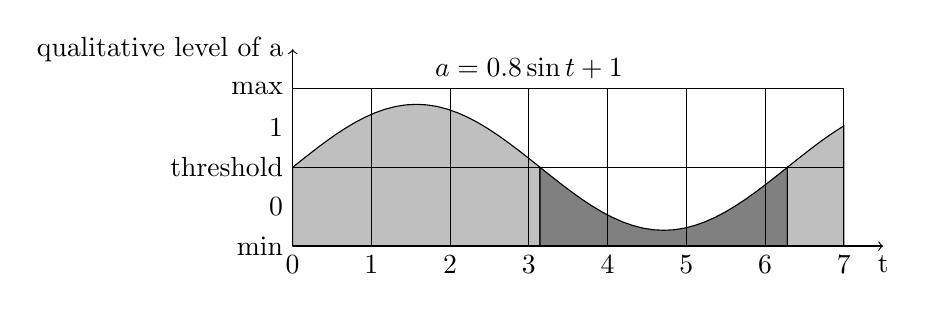
\begin{tikzpicture}
\draw[->] (0,0) -- (0,2.5);
\draw[->] (0,0) -- (7.5,0);
\draw(0,2)node[left]{max};
\draw(0,0)node[left]{min};
\draw(0,1)node[left]{threshold};
\foreach \y in {0,1} \draw(0,\y+0.5)node[left]{\y};
\foreach \x in {0,1,...,7} \draw(\x,0)node[below]{\x};
\filldraw[draw=black,fill=black!25!white]
	plot[domain=0:pi] (\x, {0.8*sin(\x r)+1})--(pi,0)--(0,0)--(0,1); 
\filldraw[draw=black,fill=gray]
	plot[domain=pi:2*pi] (\x, {0.8*sin(\x r)+1})--(2*pi,0)--(pi,0)--(pi,1); 
\filldraw[draw=black,fill=black!25!white]
	plot[domain=2*pi:7] (\x, {0.8*sin(\x r)+1})--(7,0)--(2*pi,0)--(2*pi,1); 
\draw[step=1] (0,0) grid (7,2);
\draw (7.5,0) node[below]{t};
\draw (0,2.5) node[left]{qualitative level of a};
\draw(3,2)node[above]{$a=0.8\sin t+1$};
\end{tikzpicture}
\caption{Example of variable reconstruction, former variable $a=0.8\sin t+1(t\in [0,7])$ is split into 2 variables $a_0=0.8\sin t+1(t\in (\pi,2\pi))$ (dark gray) and $a_1=0.8\sin t+1(t\in [0,\pi]\cup[2\pi,7])$ (light gray) with different domains according to the qualitative threshold}\label{varRec}
\end{figure}
After the treatment of component $a$, suppose there is another variable $b$ split into 2 variables $b_1,b_2$, then the matrix for inference of Process Hitting is done as follows:\par
Global state after discretization: $L=\{a_0,a_1\}\times \{b_0,b_1\}\ $\par
Pearson / Spearman Matrix: $r=\left[
\begin{array}{*{20}c}
1 & r_{ab}\\
r_{ba} & 1 \\
\end{array}
\right]\ 
$\par
After variable reconstruction:\par
$$r'=\left[
\begin{array}{*{20}c}
1 & r_{a_0a_1}& r_{a_0b_0}&r_{a_0b_1}\\
r_{a_1a_0} & 1& r_{a_1b_0}&r_{a_1b_1}\\
r_{b_0a_0} & r_{b_0a_1}& 1&r_{b_0b_1}\\
r_{b_1a_0} & r_{b_1a_1}& r_{b_1b_0}&1\\
\end{array}
\right]\ =\left[\begin{array}{*{20}c}
1 & 0& r_{a_0b_0}&r_{a_0b_1}\\
0 & 1& r_{a_1b_0}&r_{a_1b_1}\\
r_{b_0a_0} & r_{b_0a_1}& 1&0\\
r_{b_1a_0} & r_{b_1a_1}& 0&1\\
\end{array}\right]$$
Here, even though the size of matrix has doubled(or n times large, depending on discrete levels), as the domains of $a_0,a_1,b_0,b_1$ are not continuous and variables with same origins have no common domain, thus $r_{a_0a_1}=r_{a_1a_0}=r_{b_0b_1}=r_{b_1b_0}=0$. Also, there are probably some $r_{a_ib_j}$ equal to zero making resulted matrix sparse, which gives possibilities of optimization.
\subsection{Toy Example}
To better illustrate the whole procedure of hypothesis generation, a toy example of $4$ genes $a$, $b$, $c$ and $d$ is given below. To have an understanding of the dynamics of the system of 4 genes, we want to output regulation hypothesis for completion.\par
Input: time series data in Table \ref{TyTable1}, equitemporal measurement of 8 time units.\par
Output: regulation hypotheses for completion of over/under-approximation.\par

\begin{table}[!ht]
\centering
\begin{tabular}{*{10}{l}}
$t$&0&1&2&3&4&5&6&7&8\\
$a$&2.01&2.51&1.97&1.17&0.94&0.70&0.31&0.06&0.06\\
$b$&0.74&0.87&0.78&0.33&0.51&0.82&0.86&1.81&1.08\\
$c$&0.43&0.18&0.42&0.23&0.17&0.23&0.32&0.53&0.80\\
$d$&1.62&1.22&1.07&0.57&0.27&0.28&0.24&0.27&0.31
\end{tabular} 
\caption{Original data}\label{TyTable1}
\end{table}



\begin{table}[!ht]
\centering
\begin{tabular}{c*{8}{S}}
$t$&0&1&2&3&4&5&6&7\\
$a$&0.5&-0.54&-0.8&-0.23&-0.24&-0.39&-0.25&0.0\\
$b$&0.13&-0.09&-0.45&0.18&0.31&0.04&0.95&-0.73\\
$c$&-0.25&0.24&-0.19&-0.06&0.06&0.09&0.21&0.27\\
$d$&-0.4&-0.15&-0.5&-0.3&0.01&-0.04&0.03&0.04
\end{tabular} 
\caption{Change rates derived from original data by $x'[t]=x[t+1]-x[t]$}\label{TyTable2}
\end{table}

Change rates are obtained by subtraction, see Table \ref{TyTable2}. After data regrouping, we obtain 4 matrices with change rate of  each component respectively, 4 matrices of correlation are then calculated: \par

$$\kbordermatrix{\mbox{}&a'&b&c&d\\
a'&1.0&0.091&-0.296&-0.090   \\
b&0.091&1.0&-0.738&0.423   \\
c&-0.296&-0.738&1.0&-0.383   \\
d&-0.090&0.423&-0.383&1.0
}\qquad
\kbordermatrix{\mbox{}&a&b'&c&d\\
a&1.0&0.653&0.896&-0.976   \\
b'&0.653&1.0&0.747&-0.615   \\
c&0.896&0.747&1.0&-0.883   \\
d&-0.976&-0.615&-0.883&1.0 
}$$
$$\kbordermatrix{\mbox{}&a&b&c'&d\\
a&1.0&0.717&-0.561&-0.929   \\
b&0.717&1.0&-0.709&-0.714   \\
c'&-0.561&-0.709&1.0&0.704   \\
d&-0.929&-0.714&0.704&1.0   
}\qquad
\kbordermatrix{\mbox{}&a&b&c&d'\\
a&1.0&-0.678&0.780&0.884   \\
b&-0.678&1.0&-0.929&-0.867   \\
c&0.780&-0.929&1.0&0.907   \\
d'&0.884&-0.867&0.907&1.0   
}$$

 $r'$ is formed by taking the $i$-th line from the $i$-th matrix, which suggests the relevance between change rate of one components and the others.
$$r'=\kbordermatrix{\mbox{}&a&b&c&d\\
a&1.0&0.091&-0.296&-0.0892\\
b&0.652&1.0&0.747&-0.615\\
c&-0.561&-0.709&1.0&0.704\\
d&0.884&-0.867&0.907&1.0
}$$
We can set an arbitrary threshold e.g. 0.6, all the coefficients with their absolute value greater than 0.6 are listed below:
$$(b\ a\ 1\ 0.652),(b\ c\ 1\ 0.747),(b\ d\ 1\ -0.615),(c\ b\ 1\ -0.709)$$
$$(c\ d\ 1\ 0.704),(d\ a\ 1\ 0.884),(d\ b\ 1\ -0.867),(d\ c\ 1\ 0.907)$$
For example $(d\ b\ 1\ -0.867)$ tells that $d\xrightarrow{-}b$ is probably a good hypothesis as its absolute value of correlation coefficient is close enough to 1. Like this, a BRN model is formed, see Figure \ref{ResultBRN}. According to the configuration of Process Hitting (whether absence of regulation is regarded as counter regulation), a Process Hitting is then deduced.\par
\begin{figure}[ht]
\centering
\scalebox{1.2}{
\begin{tikzpicture}[grn]
\node[inner sep=0] (a) at (0,0) {a};
\node[inner sep=0] (b) at (2,0) {b};
\node[inner sep=0] (c) at (2,-2) {c};
\node[inner sep=0] (d) at (0,-2) {d};
%\path
%  node[elabel, below=-1em of a] {$0..2$}
%  node[elabel, below=-1em of b] {$0..1$}
%  node[elabel, below=-1em of c] {$0..1$};
\path[->]
  (b) edge node[elabel, above=-3pt] {$+1$} (a)
  (b) edge node[elabel, left=-5pt] {$+1$} (c)
  (b) edge[bend right] node[elabel, above=-3pt] {$-1$} (d)
  (c) edge[bend right] node[elabel, right=-3pt] {$-1$} (b)
  (c) edge node[elabel, above=-5pt] {$+1$} (d)
  (d) edge node[elabel, left=-3pt] {$+1$} (a)
  (d) edge node[elabel, below=-3pt] {$-1$} (b)
  (d) edge[bend right] node[elabel, below=-3pt] {$+1$} (c);
\end{tikzpicture}
}
\caption{Resulting hypotheses of the toy example}\label{ResultBRN}
\end{figure}
In fact the choice of threshold of correlation coefficients has little influence: if resulting regulations do not satisfy desired properties, we can decrease the threshold down to 0.5, because when coefficient $r =0.5$, then the 95\% prediction interval of $Y|X$ will be about 13\% smaller than the 95\% prediction interval of $Y$, i.e. Y behaves more individually than relevantly \cite{hull1927correlation}.
\section{Model Inference via a priori Constraints}
\subsection{Completion}
In the context of GLC, completion is defined as follows: given a state sequence $S$ of observation and a set of possible regulations $H$ (in the form of Process Hitting) to be verified,  find the minimum subset of $H$ such that $S$ is realizable from initial state. 
\subsection{Completion by Over-Approximation}
Over-approximation links local states with initial state: if there exists a pathway from certain state and initial state, it is said that this state is reachable in the reasoning of over-approximation. Over-approximation does not take into consideration the order of occurrence, which may make certain state unreachable (literally it over-approximates the reachability). Thus over-approximation is a sufficient condition.\par
In Figure \ref{CompOv}, the visualization of the set of possible regulations $R=\{(a,b,+),(c,a,-)\}$ is on the left. With initial state $\langle a_0,b_0,c_0\rangle$, at first $b_1$ is not reachable because of the inreachability of $a_1$, as $(c,a,-)\in R$, \ac{c_0}{a_0}{a_1} is added then $a_1$ becomes reachable which makes $b_1$ also reachable.
\begin{figure}[ht]
\centering
\begin{tikzpicture}
\coordinate (P1) at (0,0);
\node at (P1) {{\Large c}};
\coordinate (P2) at (2,0);
\node at (P2) {{\Large a}};
\coordinate (P3) at (4,0);
\node at (P3) {{\Large b}};
\coordinate (P4) at ($(P2)+(150:0.6)$);
\draw (P1) circle(0.4) ;
\draw (P2) circle(0.4);
\draw (P3) circle(0.4);
\draw [line width=1pt](30:0.5) .. controls  (1,0.7) .. (P4);
\draw [->, line width=1pt]($(P2)+(30:0.5)$) .. controls  (3,0.7) .. ($(P3)+(150:0.55)$);
\draw [line width=1pt]($(P4)+(45:0.15)$) -- ($(P4)-(45:0.15)$);
\end{tikzpicture}\qquad
\begin{tikzpicture}%[font=\scriptsize]
%\path[use as bounding box] (0,-1) rectangle (4,4);

\TSort{(0,0)}{c}{2}{l}
\TSort{(3,0)}{a}{2}{r}
\TSort{(6,0)}{b}{2}{r}
\THit{a_1}{}{b_0}{.west}{b_1}
\THit{c_0}{dashed,thick,color=red}{a_0}{.west}{a_1}


\path[bounce,bend left]
\TBounce{b_0}{}{b_1}{.west}
\TBounce{a_0}{thick,color=red}{a_1}{.west}
;
\TState{a_0,b_0,c_0}
\end{tikzpicture}
\caption{Completion by over-approximation. Dashed thick arrow represents added action.}\label{CompOv}
\end{figure}
%By means of over-approximation, if certain state is still not reachable after completion, we can say that the state is 
\subsection{Completion by Under-Approximation}
Under-approximation links local states with any possibly appearing states instead of initial state. Likewise, if there is a pathway from certain state and initial state, this state is reachable in the reasoning of under-approximation. However, all the orders of occurrence do not necessarily appear during the simulation, which suggests that this approach ``under-approximates'' the reachability. If under-approximation of certain state is true, then this state is certainly reachable. Nevertheless, the calculation of under-approximation is more complicated than over approximation, as the set of appearing states grows during the computation, former added links need to be verified with new appearing states until the set becomes stable. This process is called ``update''. \par
Take Process Hitting in Figure \ref{ExUnder} as example with initial state $\langle a_0,b_0,c_0,d_0\rangle$. Figure \ref{Under1}, Figure \ref{Under2} and Figure \ref{Under3} show the procedures of under-approximation: after two additions of actions and an update, the GLC becomes stable and $a_2$ is reachable.
\begin{figure}[!htbp]
\centering
\begin{tikzpicture}
\TSort{(3,0)}{a}{3}{l}
\TSort{(0,0)}{b}{2}{l}
\TSort{(6,0)}{c}{2}{r}
\TSort{(2,-2)}{d}{2}{b}
\THit{b_1}{}{a_0}{.north west}{a_1}
\THit{c_1}{}{a_1}{.east}{a_2}
\THit{d_0}{distance=50,out=180,in=210}{b_0}{.west}{b_1}
\THit{b_1}{}{d_0}{.north}{d_1}
\THit{d_0}{distance=100,out=-75,in=-45,dashed,thick,color=red}{c_0}{.east}{c_1}
\THit{c_1}{dashed,thick,color=red}{d_1}{.north}{d_0}


\path[bounce,bend right]	
\TBounce{a_1}{}{a_2}{.east}
\TBounce{d_1}{thick,color=red}{d_0}{.north east}
\TBounce{c_0}{thick,color=red}{c_1}{.east}
;
\path[bounce,bend left]
\TBounce{a_0}{}{a_1}{.west}
\TBounce{b_0}{}{b_1}{.west}
\TBounce{d_0}{}{d_1}{.north west}
;
\TState{a_0,b_0,c_0,d_0}
\end{tikzpicture}
\caption{Example of under-approximation. Dashed thick arrows represent added actions.}\label{ExUnder}
\end{figure}
\begin{figure}[!htbp]
\centering
\begin{tikzpicture}
\node (O1) at (0,0) {$a_0\Rsh^*a_2$};
\node[draw] (Pm1) at (-1.75,0) {$a_2$};
\draw[->] (Pm1)-- (O1);
\node (S1) at ($(O1)+(1.5,0)$){};
\draw[->] (O1) -- (S1);
\draw (S1) circle (3pt);
\node[draw] (P1) at ($(S1)+(1,1)$){$b_1$};
\node[draw] (P2) at ($(S1)+(1,-1)$){$c_1$};
\draw[->] (S1)--(P1);
\draw[->] (S1)--(P2);
\node (O2) at ($(P1)+(1.75,0)$) {$b_0\Rsh^*b_1$};
\node (O3) at ($(P2)+(1.75,0)$) {$\perp$};
\draw[->] (P1)--(O2);
\draw[->] (P2)--(O3);
\node (S2) at ($(O2)+(1.5,0)$){};
\draw (S2) circle (3pt);
\draw[->] (O2) -- (S2);
\node[draw] (P3) at ($(S2)+(1,0)$){$d_0$};
\draw[->] (S2) -- (P3);
\node (O5) at ($(P3)+(1.75,0)$) {$d_0\Rsh^*d_0$};
\draw[->] (P3)--(O5);
\node (S5) at ($(O5)+(1.5,0)$){};
\draw (S5) circle (3pt);
\draw[->] (O5) -- (S5);
\end{tikzpicture}
\caption{Under-approximation GLC of Figure \ref{ExUnder} studying the reachability of $a_2$. \fbox{$c_1$} unreachable as $(b_1\land c_1)=$ false, $a_2$ is not reachable (small circles stand for solutions and squares stand for processes)}\label{Under1}
\end{figure}

\begin{figure}[!htbp]
\centering
\begin{tikzpicture}
\node (O1) at (0,0) {$a_0\Rsh^*a_2$};
\node[draw] (Pm1) at (-1.75,0) {$a_2$};
\draw[->] (Pm1)-- (O1);
\node (S1) at ($(O1)+(1.5,0)$){};
\draw[->] (O1) -- (S1);
\draw (S1) circle (3pt);
\node[draw] (P1) at ($(S1)+(1,1)$){$b_1$};
\node[draw] (P2) at ($(S1)+(1,-1)$){$c_1$};
\draw[->] (S1)--(P1);
\draw[->] (S1)--(P2);
\node (O2) at ($(P1)+(1.75,0)$) {$b_0\Rsh^*b_1$};
\node (O3) at ($(P2)+(1.75,0)$) {$c_0\Rsh^*c_1$};
\draw[->] (P1)--(O2);
\draw[->] (P2)--(O3);
\node (S2) at ($(O2)+(1.5,0)$){};
\draw (S2) circle (3pt);
\draw[->] (O2) -- (S2);
\node (S3) at ($(O3)+(1.5,0)$){};
\draw[fill=black] (S3) circle (3pt);
\draw[->] (O3) -- (S3);
\node[draw] (P3) at ($(S2)+(1,0)$){$d_0$};
\draw[->] (S2) -- (P3);
\node[draw] (P4) at ($(S3)+(1,0)$){$d_1$};
\draw[->] (S3) -- (P4);
\node (O4) at ($(P3)+(30:1.75)$) {$d_0\Rsh^*d_0$};
\node (O5) at ($(P3)+(1.75,0)$) {$d_1\Rsh^*d_0$};
\draw[->] (P3)--(O4);
\draw[->] (P3)--(O5);
\node (O6) at ($(P4)+(-30:1.75)$) {$d_1\Rsh^*d_1$};
\node (O7) at ($(P4)+(1.75,0)$) {$d_0\Rsh^*d_1$};
\draw[->] (P4)--(O6);
\draw[->] (P4)--(O7);
\node (S4) at ($(O4)+(1.5,0)$){};
\draw (S4) circle (3pt);
\draw[->] (O4) -- (S4);
\node (S5) at ($(O5)+(1.5,0)$){$\perp$};
\draw[->] (O5) -- (S5);
\node (S6) at ($(O6)+(1.5,0)$){};
\draw[fill=black] (S6) circle (3pt);
\draw[->] (O6) -- (S6);
\node (S7) at ($(O7)+(1.5,0)$){};
\draw[fill=black] (S7) circle (3pt);
\draw[->] (O7) -- (S7);
\draw[->] ($(S7)+(0,3pt)$) -- (P1);
\end{tikzpicture}
\caption{According to possible regulation $r={(d,c,+)}\in R$, \ac{d_1}{c_0}{c_1} is added, but the reachability of under-approximation requires all the possible occurrences are realizable, e.g. transition $d_1\Rsh^*d_0$ must be realizable (filled small circles stand for new possible solutions after completion)}\label{Under2}
\end{figure}

\begin{figure}[!htbp]
\centering
\begin{tikzpicture}
\node (O1) at (0,0) {$a_0\Rsh^*a_2$};
\node[draw] (Pm1) at (-1.75,0) {$a_2$};
\draw[->] (Pm1)-- (O1);
\node (S1) at ($(O1)+(1.5,0)$){};
\draw[->] (O1) -- (S1);
\draw (S1) circle (3pt);
\node[draw] (P1) at ($(S1)+(1,1)$){$b_1$};
\node[draw] (P2) at ($(S1)+(1,-1)$){$c_1$};
\draw[->] (S1)--(P1);
\draw[->] (S1)--(P2);
\node (O2) at ($(P1)+(1.75,0)$) {$b_0\Rsh^*b_1$};
\node (O3) at ($(P2)+(1.75,0)$) {$c_0\Rsh^*c_1$};
\draw[->] (P1)--(O2);
\draw[->] (P2)--(O3);
\node (S2) at ($(O2)+(1.5,0)$){};
\draw (S2) circle (3pt);
\draw[->] (O2) -- (S2);
\node (S3) at ($(O3)+(1.5,0)$){};
\draw (S3) circle (3pt);
\draw[->] (O3) -- (S3);
\node[draw] (P3) at ($(S2)+(1,0)$){$d_0$};
\draw[->] (S2) -- (P3);
\node[draw] (P4) at ($(S3)+(1,0)$){$d_1$};
\draw[->] (S3) -- (P4);
\node (O4) at ($(P3)+(30:1.75)$) {$d_0\Rsh^*d_0$};
\node (O5) at ($(P3)+(1.75,0)$) {$d_1\Rsh^*d_0$};
\draw[->] (P3)--(O4);
\draw[->] (P3)--(O5);
\node (O6) at ($(P4)+(-30:1.75)$) {$d_1\Rsh^*d_1$};
\node (O7) at ($(P4)+(1.75,0)$) {$d_0\Rsh^*d_1$};
\draw[->] (P4)--(O6);
\draw[->] (P4)--(O7);
\node (S4) at ($(O4)+(1.5,0)$){};
\draw (S4) circle (3pt);
\draw[->] (O4) -- (S4);
\node (S5) at ($(O5)+(1.5,0)$){};
\draw[fill=black] (S5) circle (3pt);
\draw[->] (O5) -- (S5);
\node (S6) at ($(O6)+(1.5,0)$){};
\draw (S6) circle (3pt);
\draw[->] (O6) -- (S6);
\node (S7) at ($(O7)+(1.5,0)$){};
\draw (S7) circle (3pt);
\draw[->] (O7) -- (S7);
\draw[->] ($(S5)-(0,3pt)$) -- (P2);
\draw[->] ($(S7)+(0,3pt)$) -- (P1);
\end{tikzpicture}
\caption{Second step: the under-approximation GLC after completion shows $a_2$ is now reachable after adding $\acm{c_1}{d_1}{d_0}$ (filled small circles stand for new possible solutions after updates)}\label{Under3}
\end{figure}\section{Model Revision via Reachability Properties}
In \cite{inoue2011logic}, it has been shown that Boolean networks can be represented by logic programs.
In this paper, we provide a method to revise a logic program to fit temporal properties regarding reachability of partial states.
%
Such logic program can be learned from observations of state transition using LFIT algorithm in \cite{ribeiro2015learning}, but the approach restricts the model to only synchronous update scheme.
One of the benefits of synchronous modeling is computational tractability, while classical state space exploration algorithms fail on asynchronous ones.
Yet the synchronous modeling relies on quite heavy assumptions:
all genes can make a transition simultaneously and need an equivalent amount of time to change their expression level.
Even if this is not realistic from a biological point of view, it is usually sufficient as the exact kinetics and order of transformations are generally unknown.
However, the asynchronous semantics helps one to capture more realistic behaviors \cite{bernot2009}.
At a given time point, at most one single gene can change its expression level.
Non-deterministic behaviors are often observed in biological systems, e.g. cell differentiation.
From a given state, several possible behaviors can be expected as future states.
Asynchronous update scheme results in a potential combinatorial explosion to the number of states.


\subsection{Learning From Interpretation Transitions}\label{sec:lfit}
LFIT framework so far can only capture finite dynamical properties, i.e. relation at $T$-$1$ or $T$-$k$ and the system has to be synchronous deterministic.
In asynchronous systems, non-determinism can lead to loops for several times before taking a path to a certain state.
In this paper, we adapt the algorithms of \cite{ribeiro2015learning,DMTRICLP15} to capture asynchronous dynamics and extend upon this method to propose an approach allowing to fit a logic program to reachability properties.
By modifying rules of the program using logic generalization/specialization operations, we iteratively revise the program to fit a set of reachability/unreachability constraints while keeping the observation and learned rules consistent.
\subsection{Formalization}
    
	Boolean asynchronous systems can be non-deterministic, thus from the same state a variable can take both value $0$ or $1$.
	To encode this dynamics, one requires to have explicit rules for each value of a variable and the modeling of \cite{ribeiro2015learning} is not suitable.
	In \cite{DMTRICLP15}, we proposed a modeling of multi-valued synchronous systems as annotated logic program.
    This modeling can be applied to represent Boolean asynchronous systems and is recalled in the following section.
    %
	In order to represent multi-valued variables, all atoms of a logic program are now restricted to the form $var^{val}$.
	The intuition behind this form is that $var$ represents some variable of the system and $val$ represents the value of this variable.
	In annotated logics, the atom $var$ is said to be annotated by the constant $val$.
	We consider a {\it multi-valued logic program\/} as a set of {\it rules\/} of the form  
	\begin{equation}\label{multi_value}
		var^{val} \leftarrow var_1^{val_1} \wedge \cdots \wedge var_n^{val_n}
	\end{equation}
	where $var^{val}$ and $var_i^{val_i}$'s are atoms $(n \geq 1)$.
	For any rule $R$ of the form~(\ref{multi_value}), left part of $\leftarrow$ is called the {\it head\/} of $R$ and is denoted as $h(R)$,
	and the conjunction to the right of $\leftarrow$ is called the {\it body\/} of $R$.  
	We represent the set of literals in the body of $R$ of the form~(\ref{multi_value}) as $b(R)=\{var_1^{val_1},\ldots,var_n^{val_n}\}$. 
	A rule $R$ of the form (\ref{multi_value}) is interpreted as follows:
	the variable $var$ takes the value $val$ in the next state if all variables $var_i$ have the value $val_i$ in the current state.
	A state of a multi-valued program provides the value of each variable of the system and a transitions is a pair of states.
	The value of a variable in a state is called a local state.
	The set of all local state is denoted $\mathbf{LS}$.
	The subset of state is called a partial state.
	A rule $R$ matches a state $s$ when $b(R) \subseteq s$.
	A rule $R$ subsumes a rule $R'$ when $h(R)=h(R'), b(R) \subseteq b(R')$.
%
A Boolean Asynchronous system can be represented by a multi-valued logic program.
This section provides the necessary additional formalization to interpret asynchronous dynamics by such program and to learn from state transitions.

\subsection{Modeling and learning of asynchronous dynamics}\label{sec:alfit}

Due to the non-deterministic nature of asynchronous systems and its restriction to atmost one variable change per transition,
the notion of consistency, realization and successor has to be adapted as follows.

\begin{definition}[Consistency]
	Let $R$ be a rule and $E$ be a set of state transition $(I,J)$.
	$R$ is {\it consistent} with $E$ iff
	$b(R)\subseteq I$ implies $\exists (I,J) \in E, h(R) \in J$.
	A logic program $P$ is {\it consistent} with $E$ if all rules of $P$ are {\it consistent} with $E$.
\end{definition}

\begin{definition}[Program realization]
	Let $P$ be a logic program and $E$ be a set of state transitions.
	$P$ realizes $E$ if $\forall (I,J) \in E, \exists R, b(R) \subseteq I, (I \setminus J) = \{h(R)\}$.
\end{definition}

\begin{definition}[Asynchronous successors]
	Let $I$ be the current state of an asynchronous system represented by a set of multi-valued rules $S$.
	Let $T_P(I,S) = \{h(R) | R \in S, b(R) \subseteq I\}$.
	The successors of $I$ according to $S$ is
	$$T_P^{as}(I,S) = \{I \setminus \{v^{val'}\} \cup \{v^{val}\} | v^{val'} \in I, v^{val} \in T_P(I,S)\} \cup \{I \mid T_P(I,S) = \emptyset\}$$ % Self loop only for non-point atractor
\end{definition}

We now adapt the {\bf LFIT} algorithm of \cite{ribeiro2015learning} to the learning of asynchronous systems.
In synchronous case, the rules $R$ learned by {\bf LFIT} represent a necessity: $h(R)$ \textit{will} be in the next state if $R$ match the current state.
In asynchronous case, the rules represent a possibility: $h(R)$ \textit{can} be in next state if $R$ match the current state.
It allows the modeling of non-determinism: two rules $R, R'$ can have the same head variables but different values and match the same state which occurs in these case:
$h(R)=var^{val}, h(R')=var^{val'}, val \neq val'$ and $var^{val''} \in b(R), var^{val'''}\in b(R') \implies val'' = val'''$.

Like in previous versions, {\bf LFIT} takes a set of state transitions $E$ as input and outputs a logic program $P$ that realizes $E$.
In \cite{DMTRICLP15} multi-valued least specialization was used to learn multi-valued {\bf synchronous} systems dynamics.
Starting from the most general rules, least specialization allows to learn the minimal rules of such system iteratively from its state transition $(I,J) \in E$.
For every possible $var^{val}$, $var^{val} \not \in J$ the most specific rule that is not consistent, with the transition, i.e. an anti-rule, was generated: $MSR := var^{val} \leftarrow I$.
Here, for the {\bf asynchronous} case, this anti-rule is generated and the revision occurs only if $\nexists (I,J') \in E, var^{val'} \in J'$,
i.e. it is impossible to have a transition to $var^{val}$ from $I$.
Each rule of the currently learned program $P$ that subsumes such an anti-rule are specialized using least specialization.
The resulting program $P'$ is consistent and realizes all previously treated transition plus $(I,J)$.
Doing so iteratively for each transitions, the algorithm output a program $P$ which model the dynamics of the system observed in the transitions $E$.

\vspace{0.5em}
\noindent
\textbf{Asynchronous LFIT}
\vspace{-0.4em}
\begin{itemize}
	\item INPUT: $\mathcal{B}$ a set of annotated atoms and $E$ a set of transitions
	\item Initialize $P := \{var^{val} \leftarrow \emptyset \mid var^{val} \in \mathcal{B}\}$
	\item For each $(I,J) \in E$
	\begin{itemize}
		\item For each $var^{val} \in \mathcal{B}$
		\begin{itemize}
			\item If $\nexists (I,J') \in E, var^{val} \in J'$
			\item $MSR := var^{val} \leftarrow I$
			\item Extract each rule $R$ of $P$ that subsumes $MSR$: $MR := \{R \in P \mid h(R) = var^{val}, b(R) \subseteq I\}, P := P \setminus MR$
			\item For each $R \in MR$
			\begin{itemize}
				\item Compute its least specialization $P'=ls(R,MSR,\mathcal{B})$.
				\item Remove all the rules in $P'$ subsumed by a rule in $P$.
				\item Remove all the rules in $P$ subsumed by a rule in $P'$.
				\item Add all remaining rules in $P'$ to $P$.
			\end{itemize}
		\end{itemize}
	\end{itemize}
	\item OUTPUT: $P$
\end{itemize}

\begin{definition}[Consistent program]
Let $P$ be a logic program, $Re$ (resp. $Un$) be a set of reachability (resp. unreachability) properties.
$P$ is said to be {\em consistent} with $Re$ (resp. $Un$) iff
$\forall (\alpha,\omega) \in Re, \exists$ a trajectory $t$ in $P$ s.t. $\alpha.t=\omega$ and 
$\forall (\alpha,\omega) \in Un, \nexists$ a trajectory $t$ in $P$ s.t. $\alpha.t=\omega$.
\end{definition}

Specializing a rule is to add elements in the body of a rule,
thus to make the condition of a rule more difficult to be satisfied (in a more specialized situation) as the condition of firing becomes more strict.

\begin{definition}[Least Specialization of a rule]
	Let $R$ be a rule, a least specialization of $R$ is a rule $R' \in ls(R) := \{h(R) \leftarrow b(R) \cup \{var^{val}\}, \nexists var^{val'} \in b(R)\}$.
	If $R$ contains already all the variables in its body, the only way to specialize $R$ is to remove $R$.
\end{definition}

    Similarly, generalization of a rule is to remove certain elements in the body of a rule, thus to make the condition of a rule easier to be satisfied.

\begin{definition}[Least Generalization of a rule]
	Let $R$ be a rule, a least generalization of $R$ is a rule $R' \in lg(R) := \{h(R) \leftarrow b(R) \setminus \{x\},  x \in b(R)\}$.
\end{definition}

\begin{definition}[Revisable]\label{def:revisable}
	A logic program $P$ is said revisable w.r.t. a reachability (resp. unreachability) property if:
	$\exists P' \in \{(P \setminus R_P) \cup \{R' \mid R \in R_P, R' \in ls(R) \cup lg(R)\} \} \mid R_P \subseteq P\}$.
	$P$ is revisable w.r.t. to a set of property $S$:
	if their exists an ordering $S'$ of the elements of $S$ such that each $i$th revision, $0 \leq i \leq |S'|$, ($P$ being the $0$th revision) is revisable w.r.t. the $i+1$th property.
\end{definition} 

From definition \ref{def:revisable}, it follows that the revision of logic program $P$ w.r.t. a set of reachability/unreachability properties $S$ can be found (or proved to be non-existent) by brute force enumeration of all possible ordering of $S$ and trying all possible iterative revisions of $P$.
In the next section we propose an algorithm exploiting the LCG structure to restrict the search to valid ordering of the properties.
\subsection{Revision}
\label{sec:algorithm}

    In this section we propose an algorithm that exploits the previous formalization to fit a logic program to reachability properties.
    Given a set of transition $E$ of an asynchronous system $S$, a logic program $P$ is learned via the adaptation of \textbf{LFIT} of section \ref{sec:alfit}.
    When $E$ is partial, the learned program $P$ does not have the exact dynamics of $S$.
    Given a set of reachability properties $Re$ and a set of unreachability properties $Un$ of $S$, we propose an algorithm to revise $P$ so that the dynamics of $P$ satisfy $S$.
    As discussed previously, this can be done by complete brute force but here we propose a first attempt to reduce the search space.
	% TODO: detail why ordering is correct, notion of precedence and so on
    Furthermore, our aim is to find what could be considered a metric of minimal revision of $P$:
    a revision $P'$ s.t. $\nexists P'', (P''\setminus P \cap P'')\subseteq (P' \setminus P \cap P')$
   
    Specialization/generalization operations aim to revise the rule nearest to the target state in the LCG. If it is not possible, they try to revise the successor, if there is no possible solution, return $\varnothing$ to show the input logic program is not revisable. Specialization operation is limited by the observation. If $P$ after specialization can not explain all the transitions, the specialization is not admissible. %When specializing one rule, we check if all appeared transitions are explained, if not, check if there are other rules can explain it, otherwise we can not specialize it.
    Generalization is similar but without the constraint of the observation, as the observation is partial, $P$ may describe some state transitions never observed.
   
    \noindent
    \begin{minipage}{\linewidth}
    \vspace{1em}
    Specialization:
    \begin{itemize}
        \item Input: a logic program $P$, an unsatisfied element $(\alpha,\omega)$, a reachable set $Re$, an unreachable set $Un$%, a maximum addable components $k$
        \item Output: modified logic program $P$ or $\varnothing$ if not revisable
    \end{itemize}
    \begin{enumerate}
        \item $Rev\gets\{\omega\}$
        \item For each $R$ s.t. $h(R)=Rev$, for each $R'\in\{R''|R''\in ls(R)\land \nexists (I,J)\in E, \text{ s.t. } \nexists R'''\in P\cup \{R''\}\setminus \{R\}, h(R''')\in J, b(R''')\in I\}$
        \begin{itemize}
            \item If $P' \gets P \setminus \{R\} \cup \{R'\}$, $unreachable(P',\alpha,\omega$) and $P'$ satisfies all previous properties, return $P'$
        \end{itemize}
        \item $Rev\gets b(R)$ with $h(R)=Rev$ and back to step 2
        \item There is no revision for $(\alpha,\omega)$, return $\varnothing$
    \end{enumerate}
    \end{minipage}
    \noindent
    \begin{minipage}{\linewidth}
    \vspace{1em}
    Generalization:
    \begin{itemize}
        \item Input: a logic program $P$, an unsatisfied element $(\alpha,\omega)$, a reachable set $Re$, an unreachable set $Un$
        \item Output: modified logic program $P$ or $\varnothing$ if not revisable
    \end{itemize}
    \begin{enumerate}
        \item $Rev\gets\{\omega\}$
        \item For each $R$ s.t. $h(R)=Rev$, for each $R'\in lg(R)$
        \begin{itemize}
            \item If $P' \gets P \setminus \{R\} \cup \{R'\}$, $reachable(P',\alpha,\omega$) and $P'$ satisfies all previous properties, return $P'$
        \end{itemize}
        \item $Rev\gets b(R)$ with $h(R)=Rev$ and back to step 2
        \item There is no revision for $(\alpha,\omega)$, return $\varnothing$
    \end{enumerate}
    \vspace{0.1em}
    \end{minipage}
    \noindent
    \begin{minipage}{\linewidth}
    \vspace{1em}
    Complete revision:
    \begin{itemize}
        \item Input: a logic program $P$, a reachable set $Re$ and an unreachable set $Un$
        \item Output: revised logic program $P$ or $\varnothing$ if not revisable
    \end{itemize}
    \begin{enumerate}
        \item Construct the cycle-free LCGs for the elements in $Re$ and $Un$ and compute unsatisfied sets $Re'\subseteq Re$ and $Un'\subseteq Un$ which are to be revised
        \item If $Re'=\varnothing$ and $Un'=\varnothing$, return $P$
        \item Let $L=\{l_i,\ldots\}$ with $i\in Re' \cup Un'$, $l_i=\{j,\ldots\}$, with $j=(\alpha,\omega)$, $\omega \in LCG(i)$ and $ j\in Re\cup Un$ \label{step:dependency}
        \item Pick one of $l_i\in L$ of the smallest cardinality: $\nexists l_i'$, $|l_i'| < |l_i|$ \label{step:cardinality}
        \item If $l_i\cap (Re'\cup Un')\neq\varnothing$, \label{step:check}
        \begin{enumerate}
            \item Reconstruct the LCG for $i$
            \item If $l_i$ becomes consistent because of former revision, $L\gets L\setminus \{l_i\}$ and back to step 4
        \end{enumerate}
        \item If $i\in Un'$, specialize $P$ to make $i$ unreachable, if not revisable, return $\varnothing$ \label{step:specialize}
        \item Otherwise generalize $P$ to make $i$ reachable, if it is not revisable, return $\varnothing$ \label{step:generalize}
        
        \item $L\gets L\setminus\{l_i\}$ \label{step:update}
        \item If $L\neq\varnothing$ , back to step 1 \label{step:recheck}
        \item Return $P$
    \end{enumerate} 
    \vspace{0.1em}
    \end{minipage}
    
      
    The main algorithm starts with constructing the LCGs to verify $Re$ and $Un$ in order to ensure the reachability/unreachability properties to be satisfied.
    Then, for the unsatisfied properties, the program $P$ has to be revised.
    LCG can share the elements s.t. revising one can modify the others.
    By starting with the LCGs with least dependencies with others, i.e. the ones with the smallest cardinality of $l_i$, it increases the chance of partially satisfying other unsatisfied properties (step \ref{step:dependency} and \ref{step:cardinality}). 
    Then all possible revision of $P$ are generated using least specialization or generalization according to $l_i\in Re$ or $l_i \in Un$ (step \ref{step:specialize} and \ref{step:generalize}). 
    Each revision of $P$ is checked against $Re$ and $Un$ to verify that all properties satisfied by $P$ are still satisfied. 
    If new ones are satisfied, $L$ is updated accordingly (step \ref{step:check}).
    We update $P$ until there is no unsatisfied properties (step \ref{step:update} and \ref{step:recheck}).
    %As the LCGs are free of cycles, the algorithm always terminates.
    %we revise first the elements whose LCG contain least other elements in order to modify less $P$.
    Finally, if a revision of $P$ consistent with all given properties is found the algorithm terminates and outputs it.
    
\section{Summary}
Asynchronicity implies non-determinism which is meaningful to the modeling of uncertain parts in biology.
%In order to get a more realistic modeling, reachability is taken into account.
We propose a method revising the logic program learned by LFIT w.r.t. the knowledge on reachability properties. If the logic program is revisable, the revision is consistent with both state transitions and reachability information.
However, our algorithm does not guarantee the minimal revision of the logic program.
As future works, considering the metric for minimal revision and designing a related algorithm will be interesting.
%We are also developing heuristics to improve the performance of the algorithm.
Adapting more dynamical properties other than reachability also remains as our future work.